\documentclass[10pt]{article}
\usepackage[utf8]{inputenc}
\usepackage{listings}
\usepackage{float}
\usepackage{graphicx}
\usepackage{fullpage}
\usepackage{caption}
\usepackage{subcaption}
\usepackage{amsmath}
\usepackage{hyperref}
\usepackage{epstopdf}

%\renewcommand{\thesubsection}{\arabic{subsection}}
\renewcommand{\thesubsubsection}{\alph{subsubsection}}

\title{Pattern Recognition Practical 6}
\author{Group 24: \and Maikel Withagen (s1867733) \and Steven Bosch (s1861948)}
\date{\today}
\lstset{
frame=single, 
numbers=left, 
breaklines=true, 
language=Matlab,
basicstyle=\footnotesize, 
title=\lstname,
showstringspaces=false
}

\DeclareMathOperator*{\argmax}{arg\!\max}

\renewcommand{\thesection}{Assignment \arabic{section}}
\renewcommand{\thesubsection}{\arabic{subsection}}
\begin{document}
\maketitle

\section{}
\subsection{}
When we take $k=2$ the Minkowski metric is the same as the Euclidean distance between the points, which is used as error function in other clustering methods such as K-means clustering.

\subsection{}
See section \ref{Minkowski} in the appendix for our implementation.

\subsection{}
Looking at figure \ref{fig1a} we can clearly distinguish four main clusters within the data. The figures show that for higher values of t more connections are plotted. This is logical since a higher threshold permits higher distances between two points to be plotted, which overall results in more plotted connections. As for the optimal value of t, 0.05 is clearly too low, because we can see some connections within the clusters, but a lot of points that clearly belong to the clusters are left out because their distance to the other points is too high (see figure \ref{fig1b}). We can still see this for a t of 0.1, but on a smaller scale (see figure \ref{fig1c}). On the other hand a t of 0.25 is clearly too high, because multiple different clusters get connected through outliers, causing multiple clusters to be clustered together (see figure \ref{fig1f}). The same thing happens with a t of 0.2, where the two left clusters are connected (see figure \ref{fig1e}). Since this does not happen for a t of 0.15 and almost all of the points are assigned to a cluster (see figure \ref{fig1d}), this seems to be the optimal value of t. There is one point that does not get assigned to a cluster, so we will have to accept this as an outlier that does not belong to any cluster. 

\begin{figure}
  \centering
  \caption{Minkowski clustering for different threshold values.}
	\begin{subfigure}[b]{.49\textwidth}
		\includegraphics[width=\columnwidth]{Ass1_0.eps}
		\caption{}
		\label{fig1a}
	\end{subfigure}  
	\begin{subfigure}[b]{.49\textwidth}
		\includegraphics[width=\columnwidth]{Ass1_5.eps}
		\caption{}
		\label{fig1b}
	\end{subfigure}
	\quad
	\begin{subfigure}[b]{.49\textwidth}
		\includegraphics[width=\columnwidth]{Ass1_10.eps}
		\caption{}
		\label{fig1c}
	\end{subfigure}
	\begin{subfigure}[b]{.49\textwidth}
	   	\includegraphics[width=\columnwidth]{Ass1_15.eps}
	   	\caption{}
	   	\label{fig1d}
	\end{subfigure}
	\quad
	\begin{subfigure}[b]{.49\textwidth}
	   	\includegraphics[width=\columnwidth]{Ass1_20.eps}
	   	\caption{}
	   	\label{fig1e}
	\end{subfigure}
	\begin{subfigure}[b]{.49\textwidth}
		\includegraphics[width=\columnwidth]{Ass1_25.eps}
		\caption{}
		\label{fig1f}
	\end{subfigure}	
  \label{fig1.1}
\end{figure}

\section{}
\subsection{}
See section \ref{Ass2} in the appendix for our implementation.
\begin{figure}
	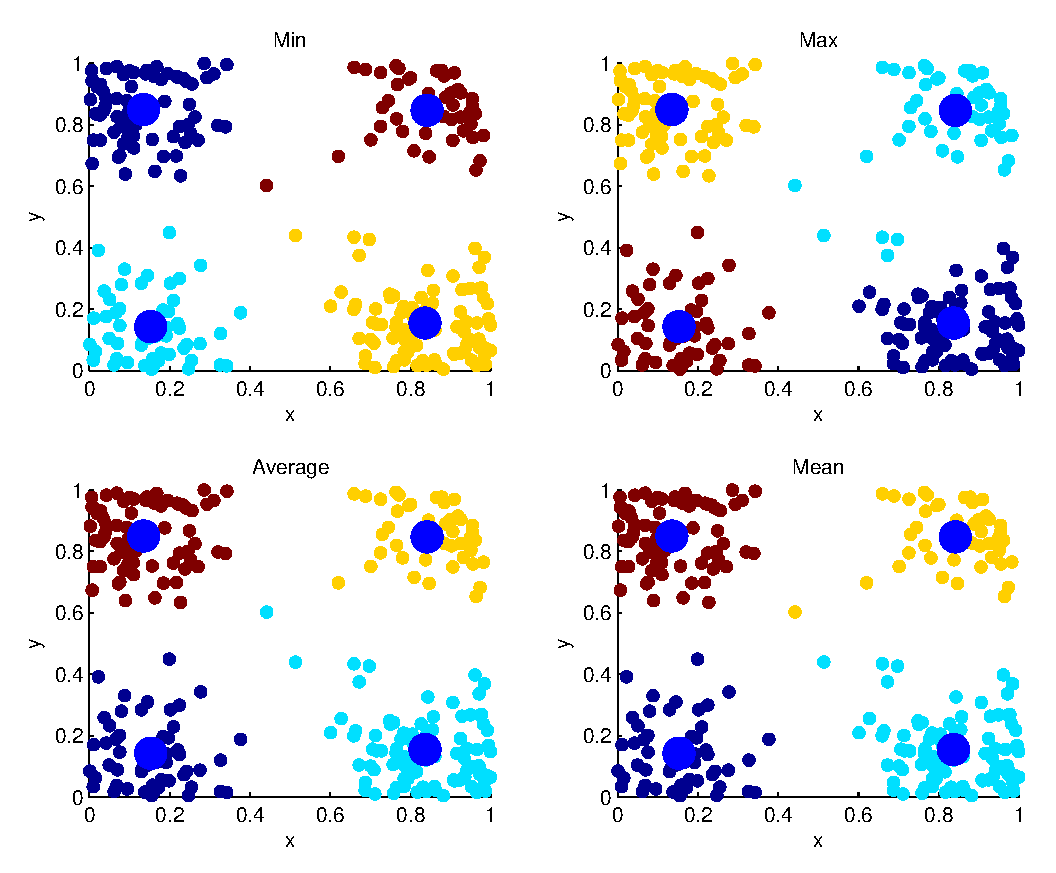
\includegraphics[width=\columnwidth]{Ass2_1.eps}
	\caption{Agglomerative hierarchical clustering using different distance functions. The big circles are the centroids per cluster.}
	\label{fig2a}
\end{figure}
\nodindent 

\subsection{}
\begin{figure}
	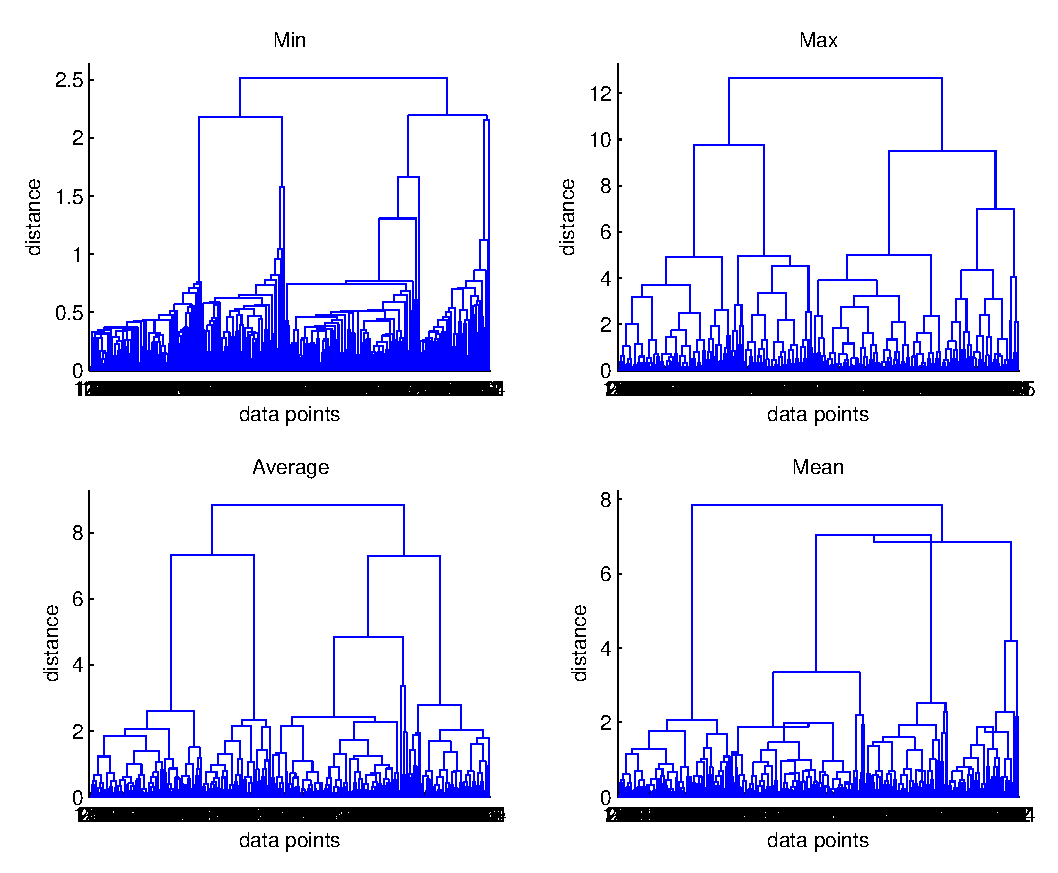
\includegraphics[width=\columnwidth]{Ass2_2.eps}
	\caption{Dendroids for the agglomerative hierarchical clustering using different distance functions.}
	\label{fig2b}
\end{figure}

\section{}
Using the code given in section \ref{Ass3} in the appendix, we computed the following J-values for the different clusterings:
\begin{table}
	\centering
	\caption{$J_e$-values for different clusters}
	\label{tab1}
	\begin{tabular}{c|c}
		Clustering & $J_e$ \\
		\hline
		$\{\{x1, x2, x3\}, \{x4, x5\}\}$ & 13.1667\\
		$\{\{x2, x3, x5\}, \{x1, x4\}\}$ & 20.6667\\
		$\{\{x4\}, \{x1, x2, x3, x5\}\}$ & 17.7500\\
		$\{\{x4, x5\}, \{x1, x2, x3\}\}$ & 13.1667\\
		$\{\{x3, x5\}, \{x1, x2, x4\}\}$ & 22.6667
	\end{tabular}
\end{table}



\newpage
\section*{Appendix}
\appendix
\section{Assignment 1}
\lstinputlisting{../Code/Ass1.m}{\label{Minkowski}}
\section{Assignment 2}
\lstinputlisting{../Code/Ass2.m}{\label{Ass2}}
\section{Assignment 3}
\lstinputlisting{../Code/Ass3.m}{\label{Ass3}}

\end{document}
